\documentclass{article}
\usepackage{amsfonts} 
\usepackage{amsmath}
\usepackage{hyperref}
\usepackage{graphicx}
\usepackage{subcaption}
\usepackage{booktabs}
\usepackage{makecell}
\usepackage{multirow}
%\usepackage{placeins}

\begin{document}


\section{Switch Types Distributions}
\begin{figure}[htbp]
\centering
\begin{subfigure}[b]{0.45\textwidth}
    \includegraphics[width=\linewidth]{pics/torus-transpositions-extended/transposition-types-complex-dim1-subposet-dim0-drop-no-switches-False.png}
    \caption{Cells dimension 0}
    \label{fig:complex1cells0}
\end{subfigure}
\hfill
\begin{subfigure}[b]{0.45\textwidth}
    \includegraphics[width=\linewidth]{pics/torus-transpositions-extended/transposition-types-complex-dim1-subposet-dim1-drop-no-switches-False.png}
    \caption{Cells dimension 1}
    \label{fig:complex1cells1}
\end{subfigure}
\vspace{0.5cm}
\begin{subfigure}[b]{0.45\textwidth}
    \includegraphics[width=\linewidth]{pics/torus-transpositions-extended/transposition-types-complex-dim1-subposet-dim0-drop-no-switches-True.png}
    \caption{Cells dimension 0 (without no switch transpositions)}
    \label{fig:complex1cells0onlyswitch}
\end{subfigure}
\hfill
\begin{subfigure}[b]{0.45\textwidth}
    \includegraphics[width=\linewidth]{pics/torus-transpositions-extended/transposition-types-complex-dim1-subposet-dim1-drop-no-switches-True.png}
    \caption{Cells dimension 1 (without no switch transpositions)}
    \label{fig:complex1cells1onlyswitch}
\end{subfigure}
\caption{The switch type distribution for $\mathbb{T}_n^{1}$}
\label{typesdistribution1}
\end{figure}

\begin{figure}[htbp]
\centering
\begin{subfigure}[b]{0.3\textwidth}
    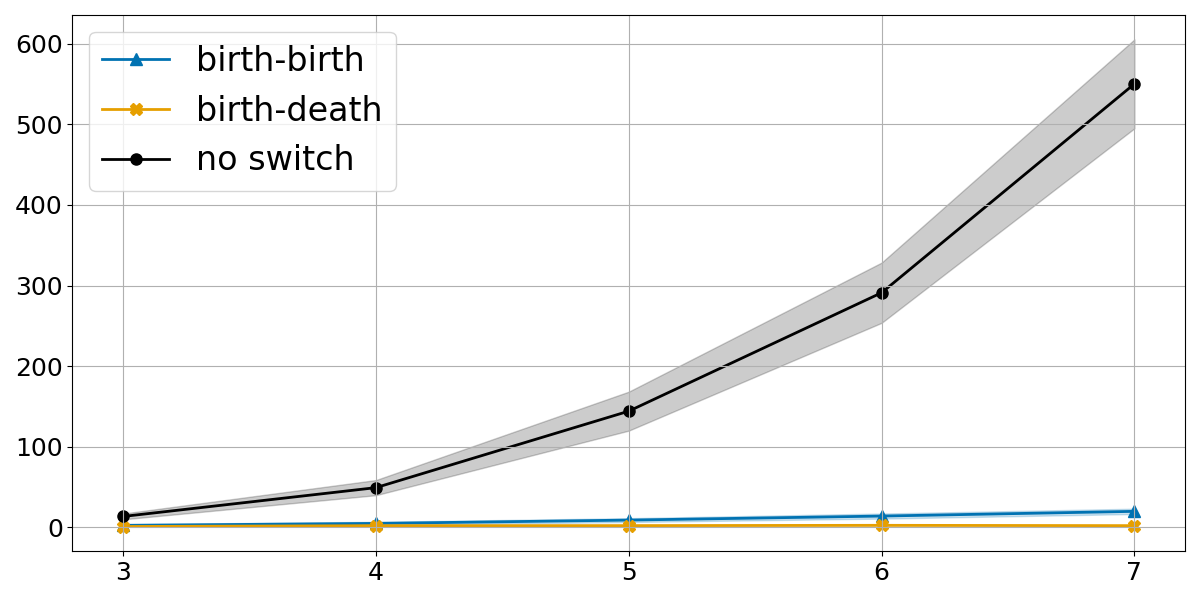
\includegraphics[width=\linewidth]{pics/torus-transpositions-extended/transposition-types-complex-dim2-subposet-dim0-drop-no-switches-False.png}
    \caption{Cells dimension 0}
    \label{fig:complex2cells0}
\end{subfigure}
\hfill
\begin{subfigure}[b]{0.3\textwidth}
    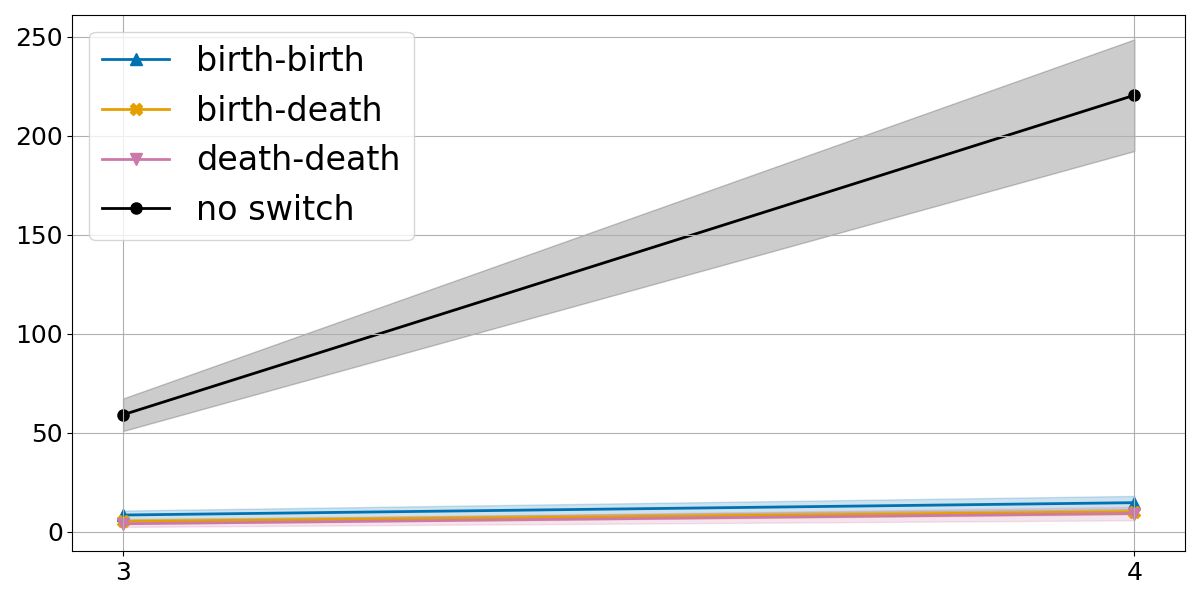
\includegraphics[width=\linewidth]{pics/torus-transpositions-extended/transposition-types-complex-dim2-subposet-dim1-drop-no-switches-False.png}
    \caption{Cells dimension 1}
    \label{fig:complex2cells1}
\end{subfigure}
\hfill
\begin{subfigure}[b]{0.3\textwidth}
    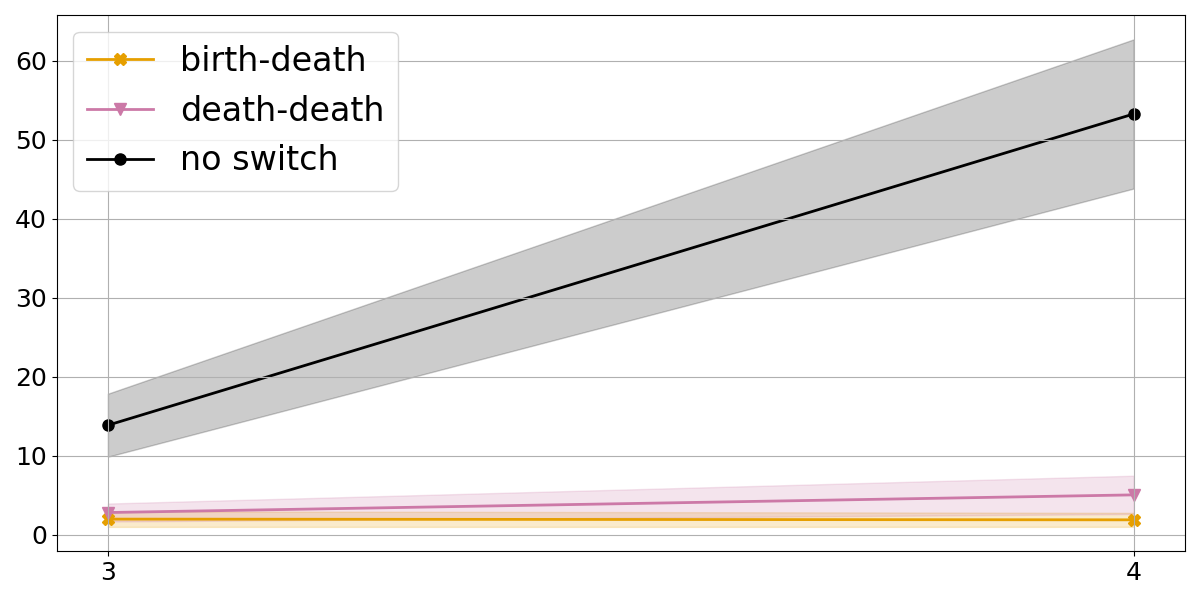
\includegraphics[width=\linewidth]{pics/torus-transpositions-extended/transposition-types-complex-dim2-subposet-dim2-drop-no-switches-False.png}
    \caption{Cells dimension 2}
    \label{fig:complex2cells2}
\end{subfigure}
\vspace{0.5cm}
\begin{subfigure}[b]{0.3\textwidth}
    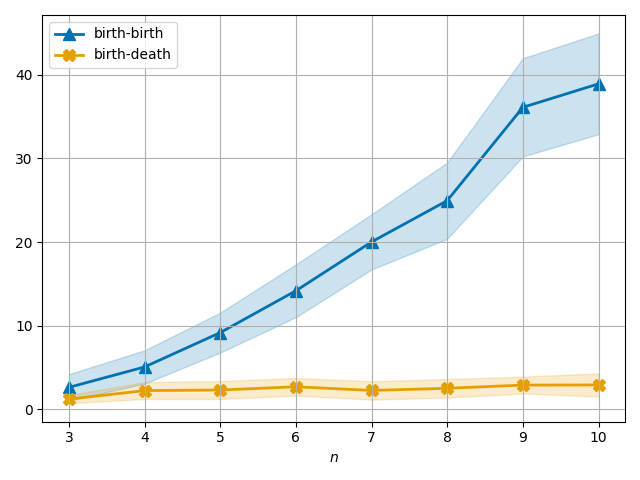
\includegraphics[width=\linewidth]{pics/torus-transpositions-extended/transposition-types-complex-dim2-subposet-dim0-drop-no-switches-True.png}
    \caption{Cells dimension 0 (without no switch transpositions)}
    \label{fig:complex2cells0onlyswitch}
\end{subfigure}
\hfill
\begin{subfigure}[b]{0.3\textwidth}
    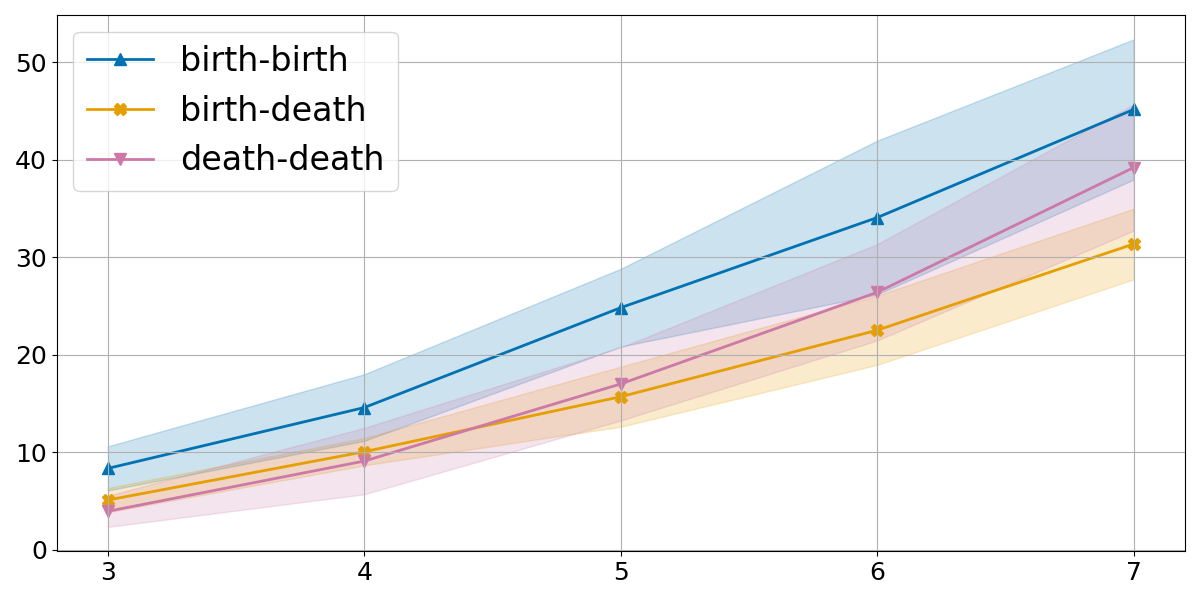
\includegraphics[width=\linewidth]{pics/torus-transpositions-extended/transposition-types-complex-dim2-subposet-dim1-drop-no-switches-True.png}
    \caption{Cells dimension 1 (without no switch transpositions)}
    \label{fig:complex2cells1onlyswitch}
\end{subfigure}
\hfill
\begin{subfigure}[b]{0.3\textwidth}
    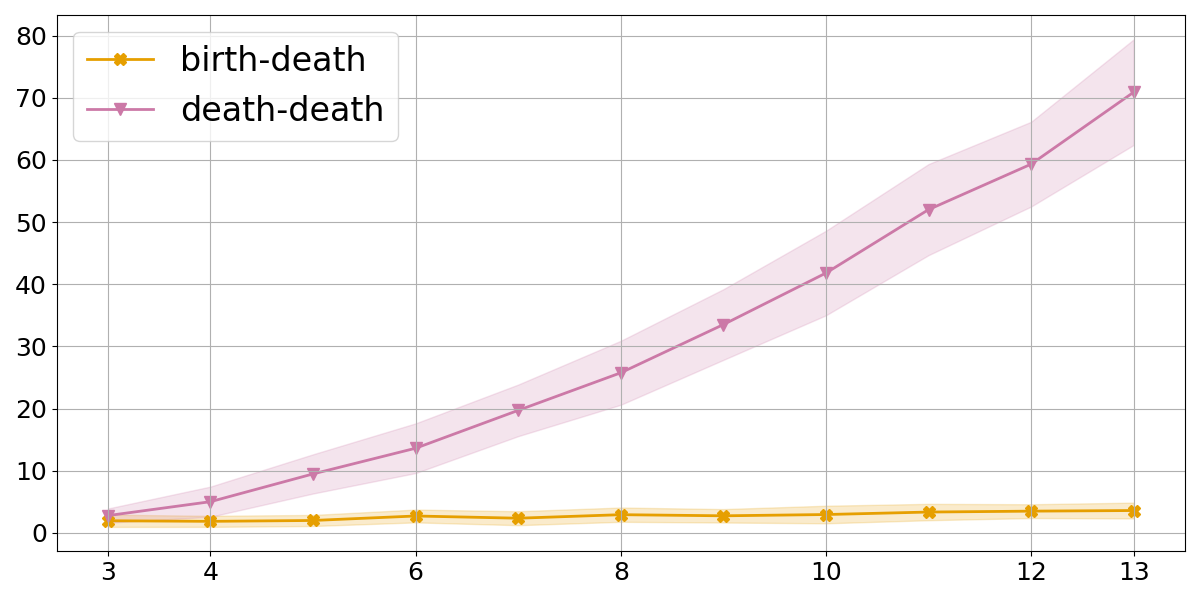
\includegraphics[width=\linewidth]{pics/torus-transpositions-extended/transposition-types-complex-dim2-subposet-dim2-drop-no-switches-True.png}
    \caption{Cells dimension 2 (without no switch transpositions)}
    \label{fig:complex2cells2onlyswitch}
\end{subfigure}
\caption{The switch type distribution for $\mathbb{T}_n^{2}$}
\label{typesdistribution2}
\end{figure}


\end{document}